 \chapter{Emotional faces in the wild database}
 \minitoc




%\section{Contributions}
%\begin{itemize}
%  \item We used LFW dataset to provide a new facial expression dataset (eLWF) by involving people in the labelling process. The new dataset contains nature facial expression rather than most of the current datasets which depending on actors facial expressions.     
%\item We show that combination of three images features extraction methods, LBP, HOG and D-SURF gives better giver stronger image description than using only one of them, and that improve classification rate with SVM and Random forests.  
%  \item We proposed a new method to identify the most relevant image regions for emotion classification and the use weights in the combination of pairwise classifiers.
%  
%  \item We describe a new weighted voting algorithm, in which the weighted predictions of classifiers trained on pairs of classes are combined with the weights learned using an evolutionary algorithm.  This method yields superior results, particularly for the hard-to-distinguish emotions.
%\end{itemize} 
 
 
 \section{Introduction}
 \label{sec:ch3_Introduction}
  Training and testing facial expression methods need databases containing human facial expressions. Researchers in the psychological field and machine learning have built various databases. The main disadvantage of most of the available datasets is that they contain unnatural expressions because the people in the databases are actors expressing their expression as they have been asked to show.   
In this thesis, we are keen to work with more natural facial expressions, to investigate how the trained model can work with various people who expressed their emotions spontaneously.

 Within the past two decades, significant effort has been made to build databases for use in facial expression recognition systems. These databases have been used for machine training and testing purposes. Some of the current databases that have mostly been used in the past two decades are the Karolinska Directed Emotional Faces (KDEF) \cite{lundqvist1998karolinska}, the AR database \citep{martinez1998ar}, the Japanese Female Facial Expression Database (JAFFE) \citep{lyons1998coding}, Cohn-Kanade facial expression databaseCohn-Kanade (CK) \citep{kanade2000comprehensive} and the extended Cohn-Kanade dataset (ck+) \citep{lucey2010extended}, the MMI facial expression database \citep{pantic2005web}, the FG-NET Facial Expressions and Emotion Database \citep{ekman1971universals, wallhoff2006facial} and the PUT Face Database \citep{kasinski2008put}.
%   CK and (CK+) have been widely used by the facial expression recognition systems.
% CK database contains 97 subjects and (CK+) 123 subjects display the basic emotions (i.e., joy, surprise, anger, fear, disgust, and sadness). 
 
  

The commonly used method of constructing these databases is to ask some actors or models to show the required facial expressions. So most researchers have used relatively unnatural datasets because in real life, natural facial expressions are different from those made by actors. The expressions of the human face are varied and show some differences between cultures and even between one person to another \citep{ekman1973cross}. Just as human sometimes find it difficult to recognise some facial expressions, machines also face the same challenges.
In this chapter, we introduce the ``Emotional Labelled Faces in the Wild'' dataset (eLFW), a citizen-labelling of 1310 faces from the Labelled Faces in the Wild data \citep{huang2007labeled}. To collect this data, we built a website and asked the citizen to label photos from the LFW dataset according to the emotional expression displayed. This chapter presents the process of the new dataset collection and labelling and shows some summary statistics of the dataset.


%____________________________________Database collection selection _____________________________________%
\section{Data collection}

 

Our work began with building a new natural facial expression database using a current database called  Labelled Faces in the Wild (LFW) \citep{LFWTech,LFWTechUpdate}. The LFW is a database of facial photographs designed for analysing the problem of unconstrained face recognition. The dataset contains 13,233 images of faces collected from the web and aligned using deep funnelling \citep{huang2012learning}. Each face has been labelled with the name of the person pictured. 1680 of the people pictured have two or more distinct photos in the database. The only constraint on these faces is that they were discovered by the Viola-Jones face detector \citep{viola2001rapid}. Figure \ref{fig:LWF} shows some examples of LWF photos.  
Since LFW photos were not labelled by emotion, our first goal was to build a website to collect some data and information from people around the world to label the facial expression.
  This website aimed to build an extensive database of real faces together with the emotion they are expressing.
Many facial photos were shown to the website visitors, and they were asked to choose the emotion that best matched the emotion being expressed by the face. They could label as many or as few as they wished.
%%%%%%%%%%%%%%%%%%%%%%%%%%%%%%%%%%%%%%%%%%%%%%%%%%%%%%%%%%%%%%%%%
\begin{figure}[t]
\centering
  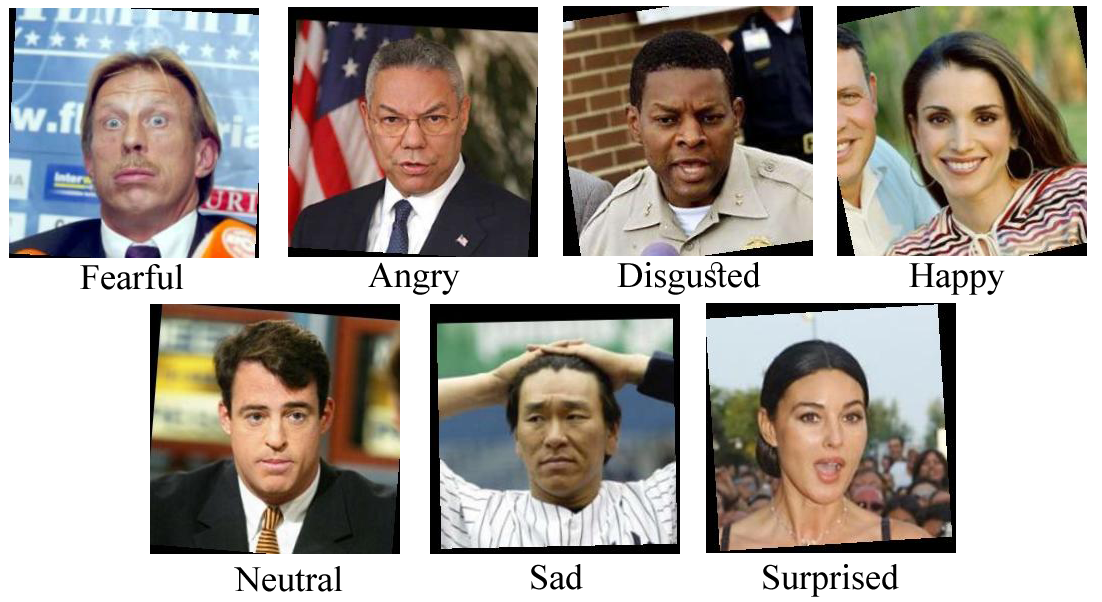
\includegraphics[width=0.8\textwidth]{Chapter3/Figs/LWF.png}
  \textbf{
    \caption{Examples of citizen labelling.}
    \label{fig:LWF}}
\end{figure}
%%%%%%%%%%%%%%%%%%%%%%%%%%%%%%%%%%%%%%%%%%%%%%%%%%%%%%%%%%%%%%%%%


To evaluate the citizen labelling we also used faces from a commonly use posed-dataset, the posed Karolinska Directed Emotional Faces(KDEF)\citep{lundqvist1998karolinska}. Figure \ref{fig:KDEF} shows some samples from it. KDEF contains a set of 4900 pictures of human facial expressions of emotion. The dataset contains 70 individuals, each displaying seven different emotional expressions, each expression being photographed (twice) from five different angles. In our experiments with KDEF, we used only frontal faces, which means 70 images for each facial expression, 490 images in total. 

%%%%%%%%%%%%%%%%%%%%%%%%%%%%%%%%%%%%%%%%%%%%%%%%%%%%%%%%%%%%%%%%%
\begin{figure}[t]
\center
  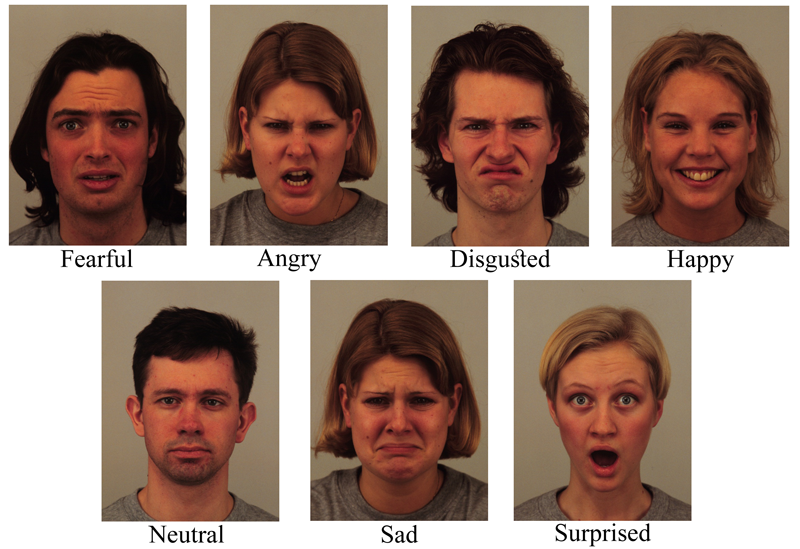
\includegraphics[width=0.8\textwidth]{Chapter3/Figs/KDEF.png}
    \textbf{\caption{Faces samples from KDEF database}\label{fig:KDEF}}
\end{figure}
%%%%%%%%%%%%%%%%%%%%%%%%%%%%%%%%%%%%%%%%%%%%%%%%%%%%%%%%%%%%%%%%%


%This thesis focuses on natural facial emotions, so we need to build a new database contains real emotions rather than not real emotions.
%An available dataset call Labelled Faces in the Wild (LFW) is a database of face photographs designed for unconstrained face recognition researches. The dataset contains 13,233 images of faces collected from the web \citep{huang2012learning}. Each face photo has been labelled with the name of the person.
% 1680 of the people pictured have two or more distinct photos in the data set\citep{huang2007labeled}. Figure \ref{fig:CH3LWF} shows some examples of LWF photos.  
%Where LFW photos are not emotionally labelled, work has started on building a website to collect some data and information from people in the world to label the facial expression, so that helps us to train machine how to recognise real emotions as human do.
%To validate our work, a current dataset called The Karolinska Directed Emotional Faces (KDEF) contains 4900 pictures of human facial expressions of emotion. 
% This website aims to build a large database of real faces together with the emotion they are expressing. Unlike most similar databases, most samples are drawn from photographs of real people on the internet rather than actors expressing the emotions. 
%Many facial photos were shown for the website visitors, and they have been asked to choose the emotion that best matches the emotion being expressed by the face. They can perform as many or as few as they wish.
%%%%%%%%%%%%%%%%%%%%%%%%%%%%%%%%%%%%%%%%%%%%%%%%%%%%%%%%%%%%%%%%%%
%\begin{figure}[tp]
%\centering
%  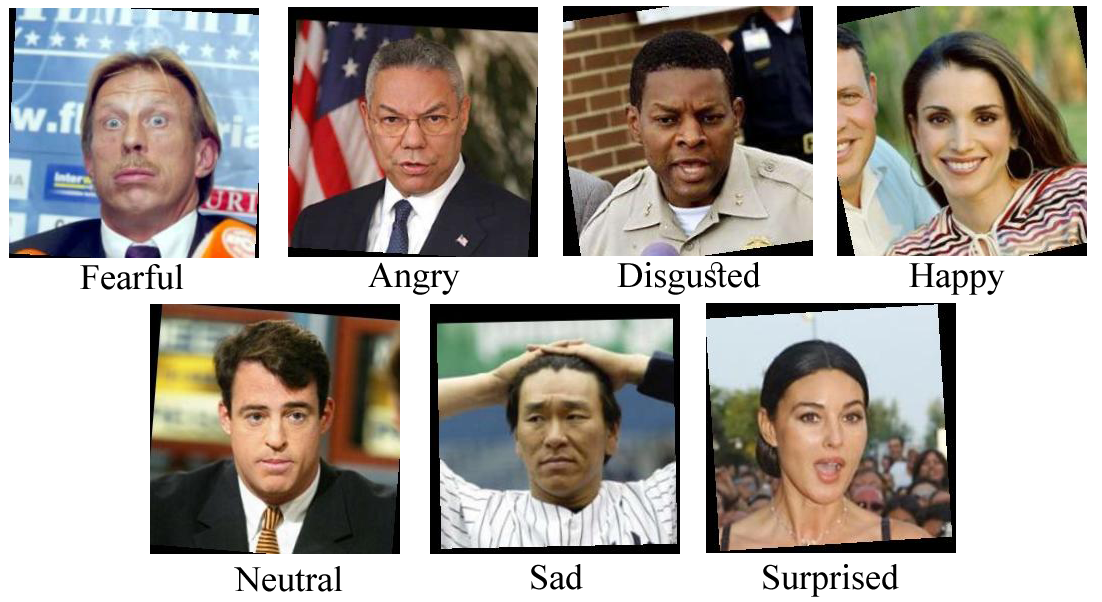
\includegraphics[width=.8\textwidth]{Chapter3/Figs/LWF.png}
%  \textbf{
%    \caption{Faces samples from LWF database}
%    \label{fig:CH3LWF}}
%\end{figure}
%%%%%%%%%%%%%%%%%%%%%%%%%%%%%%%%%%%%%%%%%%%%%%%%%%%%%%%%%%%%%%%%%%
Website visitors were shown have seen different photos chosen randomly from the two databases. The probability that displayed faces came from LFW was 0.9, so on average 1 in 10 of the faces for labelling came from KDEF data set. This allowed us to evaluate the accuracy of the citizens' labelling method.  
 For each face, people were asked to determine the emotion displayed from amongst the following: happiness, sadness, anger, fear, disgust, surprise, neutral and don't know.
 
 \begin{table}[t]
\resizebox{\textwidth}{!}{
\begin{tabular}{llllllllllll}
\multicolumn{1}{l}{Photo Name} & Happiness & Sadness & Anger & Fear & Disgust & Surprise & Contempt & Frustration & Neutral & Undefined & Entopy \tabularnewline
\hline 
Aaron\_Peirsol\_0001.jpg & 1 & 0 & 0 & 0 & 0 & 0 & 0 & 0 & 0 & 0 & 0 \tabularnewline
\hline
Colin\_Powell\_0233.jpg & 0 & 0 & 0.25 & 0 & 0.25 & 0.25 & 0 & 0 & 0.25 & 0 & 2 \tabularnewline
\hline
David\_Anderson\_0001.jpg & 0.25 & 0 & 0.25 & 0 & 0 & 0 & 0 & 0 & 0.50 & 0 & 1.5 \tabularnewline
\hline
Chloe\_Sevigny\_0001.jpg & 0.5 & 0 & 0 & 0 & 0 & 0 & 0.5 & 0 & 0 & 0 & 1\tabularnewline

\end{tabular}
}
  \caption{Voting data sample}\label{tab:label_test}

\end{table} 

 
 Since the labels assigned differed between annotators and images were presented in a randomised order, images were retained in a pool of images to be labelled until they had been assigned labels by at least four times and the consensus emotion that is the modal classification was sufficiently unequivocal.
 
 The new dataset involves useful data form each of the website visitors, and all visitors votes will be classified as the table \ref{tab:label_test}
which shows four visitors have voted on four photos, and the entropy for each photo votes. It is clear that the best entropy value for the first photo which was zero. That means the four voters have voted the same, which called the minimum entropy value. The second one, the entropy value was two, that means each voter differ from other, this case called the maximum entropy value. The third photo in the table shows that the entropy value was 1.5, which means that two votes have voted one selection, and the other two have voted in another two selections. Finally, the last photo shows two selections have been voted by fifty per cent for each, and the entropy value is one.  
  
   Ambiguous classifications were avoided by calculating the entropy of the empirical distribution of classifications. Let $p_n$ be the proportion, of citizens' votes for the $n^{th}$ emotion class ($n = 1, \ldots, 8$), then the entropy, $H = -\sum_n p_n \log_2 p_n$, measures the agreement between the annotators. The entropy is maximised when all classes are assigned in equal proportion and is minimised when images are assigned to only a single class.  We, therefore, kept an image in the pool of images to be labelled until the entropy of the citizens' assignments was less than $1$ bit.  Images that did not receive an unambiguous classification after 15 votes, and images for which the consensus was ``don't know'' were rejected.
 

 In addition to the LFW images, approximately one in ten images presented to the citizens was a KDEF posed image. This allowed us to check the integrity of individual annotators and, as discussed below, investigate human performance on the KDEF data.  As Table \ref{DatabaseNumbers} shows, the KDEF images were, unsurprisingly, easier than the LFW data for citizens to classify, requiring fewer votes to reduce the entropy below the acceptance threshold.
 
% The citizens classified the 278 KDEF photos as shown in table \ref{VotedKDEF}, which were distributed as 49 fear, 35 anger, 42 disgust, 47 happy, 35 neutral, 34 sad and 36 surprised. The overall agreement of citizens with the KDEF labelling was 80.6\%. As the confusion matrix in Table \ref{VotedKDEF} shows, there was complete agreement with the KDEF labelling for happy and neutral facial expressions, but only 42.9\% for fear (confused principally with disgust and surprise); 77.8\% for surprise (confused principally with fear  and anger); and 78.6\% for disgust (confused principally with sadness and surprise).
%Figure \ref{fig:KDEF-vs-citizen} shows examples of faces for which the citizen consensus differed from the KDEF labelling.
%


% \begin{table}[tb]
%  \centering
%  \caption{Summary statistics for the eLFW database.}
%  \fontsize{5pt}{5pt}
%  \label{DatabaseNumbers}
%  \begin{tabular}{lr@{\hspace{4mm}}r}
%    \toprule
%     & KDEF & LFW \\ \cline{2-3}
%    Number of accepted images & 278 & 1310 \\ 
%    Mean number of votes for accepted  images\qquad\qquad & 4.989 & 7.203 \\
%    Average entropy for accepted images (bits) &    0.668 & 0.905\\
%\bottomrule
%\end{tabular}
%\end{table}

We used ASP.Net to build the website, and SQL Server to build the database. ASP.NET is a development framework for building web pages and websites with HTML, CSS, JavaScript and server scripting, while SQL Server is an efficient relational database management system (RDBMS) form Microsoft. 


Two versions of the website have been designed to be more usable for all users, those using PCs as shown in figure \ref{fig:webisteversion}, smartphones and tablet as shown in figure \ref{fig:phoneversion}. The website automatically redirects users to the appropriate version. This website has been tested many times, to make sure is it easy to use by users. 

%%%%%%%%%%%%%%%%%%%%%%%%%%%%%%%%%%%%%%%%%%%%%%%%%%%%%%%%%%%%%%%%%

\begin{figure}[t]
\centering
\begin{subfigure}{.6\textwidth}
  \centering
  \fbox{\includegraphics[width=1\textwidth]{Chapter3/Figs/Fig15.jpg}}
  \caption{large screen version}
  \label{fig:webisteversion}
\end{subfigure}%
\begin{subfigure}{.525\textwidth}
  \centering
 \fbox{ \includegraphics[width=0.3\textwidth]{Chapter3/Figs/Fig16.jpg}}
  \caption{Mobile version}
  \label{fig:phoneversion}
\end{subfigure}
\caption{Screenshots two versions of the emotional faces website}
\label{fig:Site_versions}
\end{figure}


%
%
%\begin{figure}[tp]
%\centering
%  \fbox{\includegraphics[width=1\textwidth]{Chapter4/Figs/Fig15.jpg}}
%  \textbf{
%    \caption{Screenshot of large screen version of the emotional faces website}
%\label{fig:webisteversion}}
%\end{figure}
%%%%%%%%%%%%%%%%%%%%%%%%%%%%%%%%%%%%%%%%%%%%%%%%%%%%%%%%%%%%%%%%%%
%
%The website's compatibility was tested on  popular browsers such as Internet Explorer, Google Chrome, Firefox, Safari and Opera.
%%%%%%%%%%%%%%%%%%%%%%%%%%%%%%%%%%%%%%%%%%%%%%%%%%%%%%%%%%%%%%%%%%
%\begin{figure}[tp]
%\centering
% \fbox{ \includegraphics[width=0.3\textwidth]{Chapter4/Figs/Fig16.jpg}}
%  \textbf{
%    \caption{Screenshot of mobile version of the emotional faces website}
%\label{fig:phoneversion}}
%\end{figure}
%%%%%%%%%%%%%%%%%%%%%%%%%%%%%%%%%%%%%%%%%%%%%%%%%%%%%%%%%%%%%%%%%%

\section{Summary of Citizens' classification}

 Table \ref{DatabaseNumbers} shows summary statics of the new data set collection.
135 visitors correctly voted (1588) photos from both datasets, KDEF and LWF.  To achieve low entropy values,  the citizens made applicability seven votes on average on each LWF image and only five votes for KDEF.  The average votes entropy for accepted LWF photos is 0.905, and for KDEF is  0.668. It is clear that, unsurprisingly, KDEF images were easier to classify than LWF images.


%%%%%%%%%%%%%%%%%%%%%%%%%%%%%%%%%%%%%%%%%%%%%%%%%%%%%%%%%%%%%%%%

\begin{table}[t]
\centering
\scriptsize    
\textbf{
\caption{Some numbers from the built database}\label{DatabaseNumbers}}
\begin{tabular}{@{}ll@{}}
\midrule
Users have voted \hspace{5.4cm}  & 135 \\
Accepted LWF photos & 1310 \\
Accepted KDEF photos & 278 \\
Mean number of votes for accepted KDEF photos & 4.989 \\
Average votes entropy for accepted KDEF photos &    0.668 \\
Mean number of votes for accepted LWF photos &     7.203 \\
Average votes entropy for accepted LWF photos &    0.905 \\
\midrule
\end{tabular}
\end{table}
%%%%%%%%%%%%%%%%%%%%%%%%%%%%%%%%%%%%%%%%%%%%%%%%%%%%%%%%%%%%%%%%



%%%%%%%%%%%%%%%%%%%%%%%%%%%%%%%%%%%%%%%%%%%%%%%%%%%%%%%%%%%%%%%%%

\begin{table}[t]
\centering    
\caption{Confusion matrices for the citizens' performance on KDEF images. True classes are shown by rows, with assigned classes in columns. FE: fear; AN: anger; DI: disgust; HA: happiness; NE: neutral; SA: sadness; SU: surprise.}
\label{VotedKDEF}
      \resizebox{.70\textwidth}{!}{%
\begin{tabular}{@{}|l|c|c|c|c|c|c|c|@{}}
\toprule
            & \textbf{FE}    & \textbf{AN}    & \textbf{DI}    & \textbf{HA} & \textbf{NE} & \textbf{SA}    & \textbf{SU}    \tabularnewline \midrule
\textbf{FE} & \textbf{0.429} & 0.020          & 0.347           & 0.000           & 0.000           & 0.061          & 0.143          \tabularnewline \midrule
\textbf{AN} & 0.057          & \textbf{0.800} & 0.086           & 0.000           & 0.000           & 0.029          & 0.029           \tabularnewline \midrule
\textbf{DI} & 0.000          & 0.024          & \textbf{0.786}  & 0.000           & 0.000           & 0.048          & 0.143           \tabularnewline \midrule
\textbf{HA} & 0.000          & 0.000          & 0.000           & \textbf{1.000}  & 0.000           & 0.000          & 0.000           \tabularnewline \midrule
\textbf{NE} & 0.000          & 0.000          & 0.000           & 0.000           & \textbf{1.000}  & 0.000          & 0.000           \tabularnewline \midrule
\textbf{SA} & 0.059          & 0.000          & 0.059           & 0.000           & 0.000           & \textbf{0.853} & 0.029            \tabularnewline \midrule
\textbf{SU} & 0.139          & 0.056          & 0.000           & 0.000           & 0.000           & 0.028          & \textbf{0.778}  \tabularnewline \bottomrule
\end{tabular}}
\end{table}
%%%%%%%%%%%%%%%%%%%%%%%%%%%%%%%%%%%%%%%%%%%%%%%%%%%%%%%%%%%%%%%%%
%\begin{table}[H]
%\centering    
%\textbf{
%\caption{Confusion matrices for the citizens' performance on KDEF images.}\label{VotedKDEF}}
%
%\selectfont
%\begin{tabular}{@{}|l|c|c|c|c|c|c|c|@{}}
%\hline
%            & \textbf{FE}    & \textbf{AN}    & \textbf{DI}    & \textbf{HA} & \textbf{NE} & \textbf{SA}    & \textbf{SU}    \\ \hline
%\textbf{FE} & \textbf{0.429} & 0.020          & 0.347           & 0.000           & 0.000           & 0.061          & 0.143 \\ \hline
%\textbf{AN} & 0.057          & \textbf{0.800} & 0.086           & 0.000           & 0.000           & 0.029          & 0.029 \\ \hline
%\textbf{DI} & 0.000          & 0.024          & \textbf{0.786}  & 0.000           & 0.000           & 0.048          & 0.143 \\ \hline
%\textbf{HA} & 0.000          & 0.000          & 0.000           & \textbf{1.000}  & 0.000           & 0.000          & 0.000 \\ \hline
%\textbf{NE} & 0.000          & 0.000          & 0.000           & 0.000           & \textbf{1.000}  & 0.000          & 0.000 \\ \hline
%\textbf{SA} & 0.059          & 0.000          & 0.059           & 0.000           & 0.000           & \textbf{0.853} & 0.029  \\ \hline
%\textbf{SU} & 0.139          & 0.056          & 0.000           & 0.000           & 0.000           & 0.028          & \textbf{0.778}  \\ \hline
%\end{tabular}
%\end{table}
%%%%%%%%%%%%%%%%%%%%%%%%%%%%%%%%%%%%%%%%%%%%%%%%%%%%%%%%%%%%%%%%%
%%%%%%%%%%%%%%%%%%%%%%%%%%%%%%%%%%%%%%%%%%%%%%%%%%%%%%%%%%%%%%%%%


%
%%%%%%%%%%%%%%%%%%%%%%%%%%%%%%%%%%%%%%%%%%%%%%%%%%%%%%%%%%%%%%%%%%
%\begin{table}[H]
%\centering
%\caption{Some examples show how people voted the KDEF faces by different emotions than which they have been labelled.}
%
%\label{MissedClassifed}
%\begin{tabular}{|l|l|l|}
%\hline
%Image & Originally labelled & People voted \tabularnewline\hline
%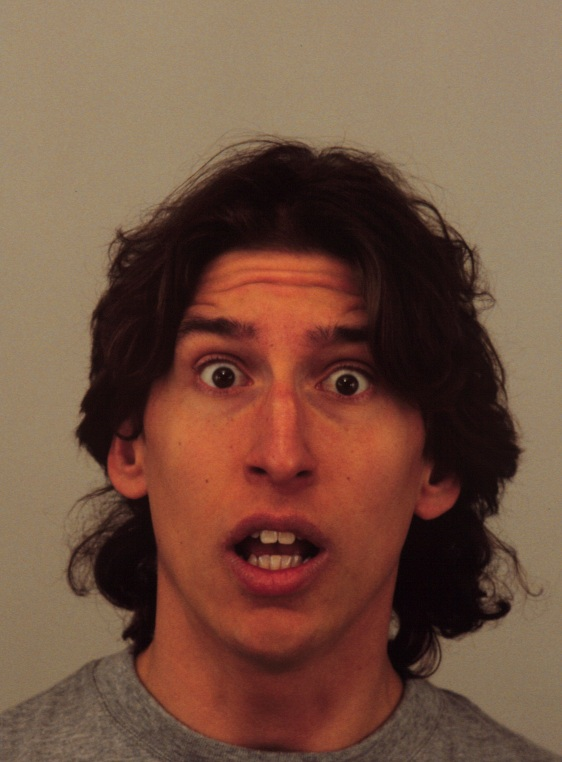
\includegraphics[valign=m,scale=0.075]{Chapter4/Figs/MissedFear.JPG} & {\large Fear} & {\large Surprised}  \tabularnewline
%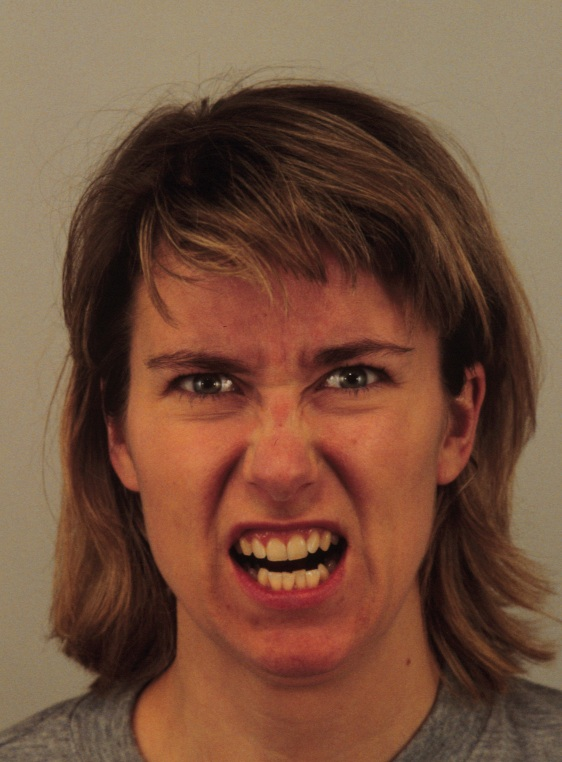
\includegraphics[valign=m,scale=0.075]{Chapter4/Figs/MissedAnger.JPG} & {\large Anger} & {\large Disgusted} \tabularnewline
%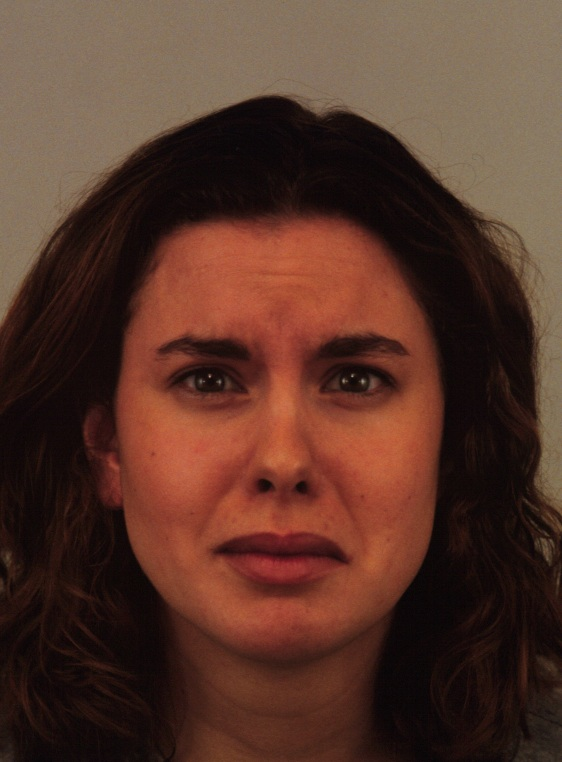
\includegraphics[valign=m,scale=0.075]{Chapter4/Figs/MissedSad.JPG} & {\large Sad}  & {\large Fear} \tabularnewline\hline
%\end{tabular}
%\end{table}
%%%%%%%%%%%%%%%%%%%%%%%%%%%%%%%%%%%%%%%%%%%%%%%%%%%%%%%%%%%%%%%%%%
The citizens classified the 278 KDEF photos as shown in Table \ref{VotedKDEF}, which were distributed as: 49 fear, 35 anger, 42 disgust, 47 happy, 35 neutral, 34 sad and 36 surprised. The overall agreement of voters with the KDEF labelling was 80.6\%. As the confusion matrix in Table \ref{VotedKDEF} shows, there was complete agreement with the KDEF labelling for happy and neutral facial expressions, but only 42.9\% for fear (confused principally with disgust and surprise), 77.8\% for surprise (confused principally with fear  and anger), and 78.6\% for disgust (confused principally with sadness and surprise). 
The mean number of votes and average votes entropy for accepted KDEF photos values where larger than those for eLFW, which mean that it was easier for citizens to classify the KDEF images than the eLFW. 
Figure \ref{fig:KDEF-vs-citizen} shows examples of faces for which the citizen consensus differed from the KDEF labelling. We conclude that some facial expressions are similar to each other, and even humans may be confused while determining what the expression is, so machines may face the same problems while recognising the expression.


\begin{figure}[H]
  \centering
  \begin{tabular}[t]{ccc}
    Fear & Anger & Sad \\
    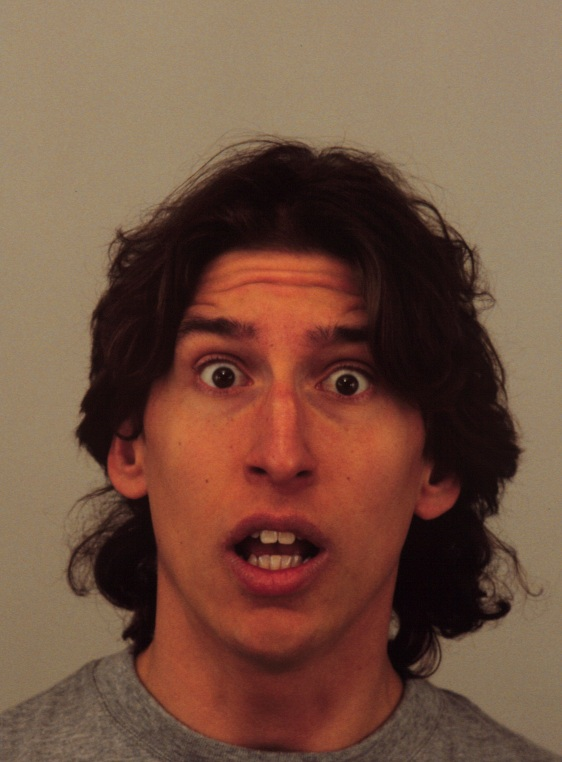
\includegraphics[scale=0.2]{Chapter4/Figs/MissedFear}
         &
   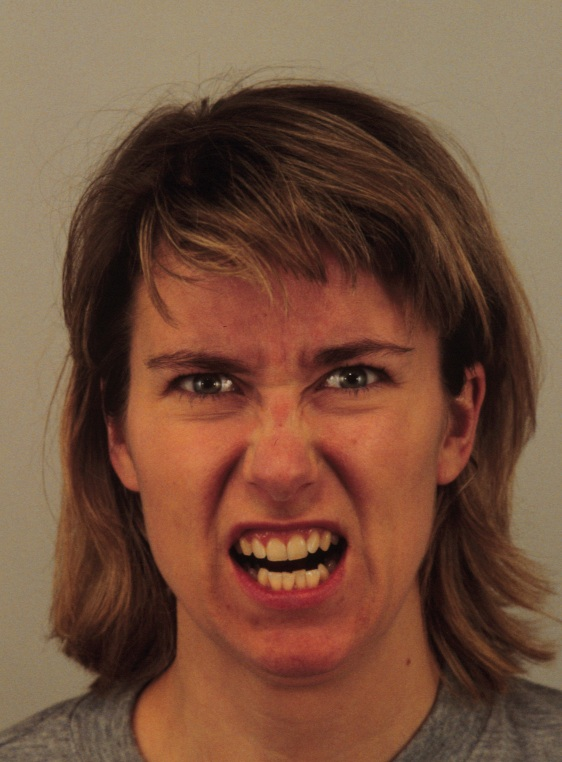
\includegraphics[scale=0.2]{Chapter4/Figs/MissedAnger}
         &
   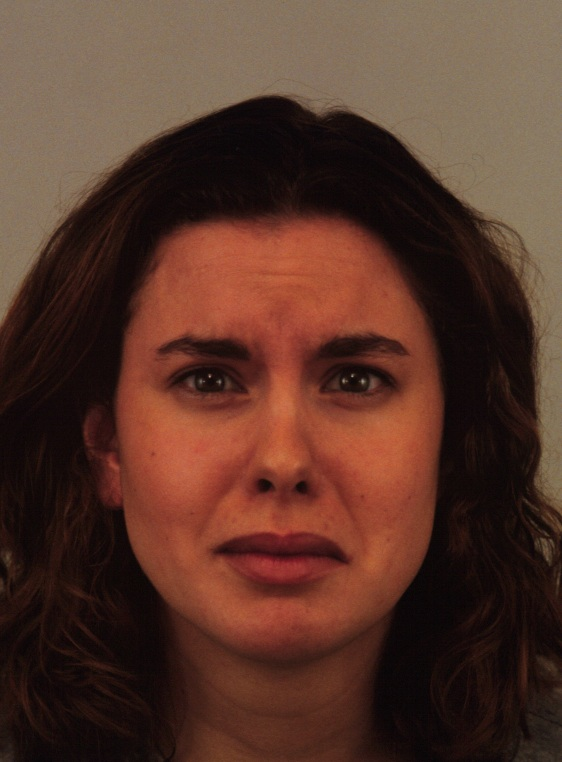
\includegraphics[scale=0.2]{Chapter4/Figs/MissedSad} \\
   Surprised  & Disgusted & Fear
  \end{tabular}
  \caption{Examples of faces for which citizens' votes differ from the KDEF labelling.  KDEF labels are shown above each image with the citizens' consensus below.}
  \label{fig:KDEF-vs-citizen}
\end{figure}



\section{Summary}
The lack of unposed labelled data has hampered work on machine recognition of emotional expressions.  In this chapter, we have described the new emotional Labelled Faces in the Wild (eLFW) database, a citizen labelling of LFW faces.  After labelling by citizens, the eLFW database comprises 190 fear images, 120 anger, 160 disgust, 330 happy, 240 neutral, 200 sad and 70 surprise images.
 The new data set enables us to evaluate the proposed texture based emotions classification on realistic data.  
\label{sec:ch3_Summary}





%____________________________________END Database collection selection _____________________________________%
